\begin{chapter}{Protótipo}
O acionador baseado em sopro foi desenvolvido com a intenção de ser
\textit{open-source} e de baixo custo, para que mais pessoas possam ter acesso
a essa ferramenta que pode ser utilizada como método alternativo para o clique
do \textit{mouse}. O circuito do protótipo desenvolvido neste trabalho é mostrado 
na Figura~\ref{fig:circuito}

\begin{figure}[!h]
	\centering
	\begin{minipage}[c]{\textwidth}
	\centering
	\includegraphics[width=0.9\linewidth]{fig/acionador}
	\caption{Esquemático do acionador baseado em sopro.}
	\label{fig:circuito}
	\end{minipage}
\end{figure} 

O princípio de funcionamento do acionador externo proposto é relativamente
simples. A percepção do sopro é realizada graças ao piezo encapsulado em um
disco redondo que fica acoplado na parte superior do dispositivo. Quando o
usuário realiza o sopro diretamente no piezo, há um estresse mecânico que produz
uma diferença de potencial elétrica nas extremidades do material piezoelétrico. 
Através dessa tensão produzida no piezo, é possível gerar um evento de
clique de \textit{mouse} no computador. O resistor colocado em paralelo com o
piezo é responsável por determinar a sensibilidade com que o transdutor gera
tensão após ser submetido a algum tipo de estresse mecânico. Portanto, quanto
maior o valor de resistência do resistor, maior será a sensibilidade do piezo.
No protótipo desenvolvido, utilizou-se um resistor de 10~M\si{\ohm}, o que
proporcionou uma boa sensibilidade no piezo. Resistores com valores de
resistência maiores que 10~M\si{\ohm}, como 15~M\si{\ohm}, 20~M\si{\ohm} e
30~M\si{\ohm}, também foram testados, contudo a sensibilidade com resistências
maiores que 15~M\si{\ohm} deixava o transdutor muito suscetível a detectar
estresses mecânicos com intensidades não desejadas. Já a
resistência de 
15~M\si{\ohm} não apresentou diferenças significativas na sensibilidade do piezo 
em relação ao resistor de 10~M\si{\ohm}, portanto, a resistêcia de 10~M\si{\ohm}
foi escolhida. 

O sinal da tensão gerado nas extremidades do material piezoelétrico é analógico.
Contudo, como o clique do \textit{mouse} possui uma natureza binária, pois há
apenas dois estados possíveis (clique ativado e clique não ativado), não
seria possível utilizar diretamente essa tensão produzida como forma de ativação
do clique devido a grande quantidade de ruído que esse sinal possui. Por isso 
houve a necessidade de digitalizar a saída do acionador.

A solução encontrada para realizar a tarefa de ``converter'' o sinal analógico
do acionador para um sinal digital, foi a utilização de um amplificador
operacional LM358. Esse componente eletrônico possui a função de comparar duas
tensões que determinam a saída do acionador. Há uma tensão de referência, que
pode ser variável graças a um potenciômetro de 10~k\si{\ohm}, e a tensão
produzida pelo transdutor piezo. O amplificador operacional atua, neste caso,
como um comparador de tensões na configuração não inversora. Quando a tensão de
referência é superior a tensão do piezo, a saída do amplificador é de nível
lógico baixo. Contudo, quando a tensão de referência é inferior a tensão do
piezo, a saída do amplificador é de nível lógico alto. Não há possibilidade da
saída do amplificador ser diferente desses dois casos. Dessa forma, a leitura do
sinal de tensão produzido pelo sopro, com o auxílio do piezo, é binária, o que
ajuda a implementar a emulação dos eventos de clique. É importante ressaltar
que, como o valor de referência pode ser ajustável, graças ao potenciômetro,
esse componente também atua como um ferramenta de ajuste de sensibilidade. Sendo
assim, a intensidade do sopro necessária para que a saída do amplificador seja
de nível lógico alto, configurando assim um clique, pode ser determinada pela
tensão de referência ajustada pelo potenciômetro.

Como um dos objetivos do acionador é ser de baixo custo, a comunicação entre o
acionador desenvolvido e o computador é realizada através da interface de áudio
P2 Jack. Para gerar um pulso na interface de áudio, basta curto-circuitar o pino
de GND com o \textit{Right} e \textit{Left} do P2 Jack do acionador. Para fazer
isso, foi necessário a utilização de uma porta lógica inversora do componente
SN7404, ilustrado na Figura~\ref{fig:sn7404}. Essa porta lógica captura o sinal
da saída do LM358 somente quando a saída do amplificador é de nível lógico alto,
pois a saída desse componente também é utilizado como alimentação do SN7404.
Portanto, quando a saída do amplificador é de nível lógico baixo, o inversor não
funciona, pois não há tensão suficiente para alimentar esse componente. Quando a
saída do LM358 é de nível lógico alto, o inversor é alimentado com uma tensão
suficiente para realizar o funcionamento correto. Essa tensão é utilizada como
entrada do SN7404 que inverte o sinal de entrada para nível lógico baixo. A
saída do inversor é conectada nos pinos  \textit{Right} e \textit{Left} do P2
Jack --- que estão curto circuitados --- gerando um pulso na entrada da
interface de áudio do computador. A partir desse pulso reconhecido pelo
computador é possível realizar a implementação da emulação dos evento de clique
do \textit{mouse}.

\begin{figure}[!h]
	\centering
	\begin{minipage}[c]{\textwidth}
	\centering
	\includegraphics[width=0.45\linewidth]{fig/sn7404}
	\caption{Circuito interno do componente sn7404.}
	\label{fig:sn7404}
	\end{minipage}
\end{figure} 

É importante ressaltar que a tensão de saída do amplificador operacional, quando
está em nível lógico alto, é bem próximo de 9~V. Essa tensão é superior a tensão
recomendada (5,5~V) pela fabricante do componente~\cite{7404}.  Para diminuir
essa tensão para a recomendada, foi utilizado um LED vermelho em série com um
resistor de 300~\si{\ohm}. Quando a saída do amplificador é de nível lógico
alto, há uma queda de tensão do cátodo do LED que é suficiente para alimentar o
inversor. Sendo assim, além de ser utilizado como divisor de tensão, o LED
também funciona como um \textit{feedback} visual, indicando quando o acionador
foi ativado pelo sopro do usuário.  


\begin{section}{Confecção da Placa de Circuito Impresso}

Para a construção da placa do acionador baseado em sopro, o \textit{software}
KiCad foi utilizado como ferramenta para desenvolver o \textit{layout} do
circuito do acionador. Todo o projeto da construção do acionador proposto está
disponível em~\cite{ErickGit} para que qualquer pessoa possa acessar o projeto
e, se desejar, construir seu próprio acionador. É importante ressaltar que
alguns componentes, como o piezo, não possuíam biblioteca nativa no Kicad. Por
isso foi necessário desenvolver uma biblioteca para cada um desses componentes.

Após a construção do \textit{layout} do circuito no Kicad etapa de confecção da
placa foi iniciada. A técnica de transferência térmica, um método bem primitivo,
porém bastante prático e barato, foi utilizada. O circuito é impresso em papel
fotográfico em uma impressora a \textit{laser} na melhor qualidade possível. Em
seguida, o circuito é transferido para uma placa de fenolite ou de fibra de
vidro através de um processo térmico, onde a placa é pressionada por uma
superfície em temperatura relativamente alta. No caso do protótipo construído
neste trabalho, um ferro de passar roupa foi utilizado para realizar esse
processo térmico. É importante pressionar bastante o ferro de passar roupa
contra a placa e realizar movimentos em todas as direções a fim de transferir
totalmente o \textit{layout} do circuito desenhado para a placa. Após o processo
térmico, se algum trecho do circuito não for transferido para a placa, é
possível corrigir, com um pincel marcador permanente de CD/DVD, as trilhas não
transferidas do circuito. 

O processo seguinte a transferência do circuito para a placa é a sua corrosão.
Para isso, é utilizada uma solução de percloreto de ferro. Essa solução é
muito fácil de ser encontrada, pois muitas lojas de eletrônica vendem esse
produto. Geralmente, o percloreto de ferro é vendido em pó, porém é necessário
apenas misturar o produto com água para obter a solução desejada. A placa com o
circuito recém transferido é mergulhada nessa solução e todo o cobre da placa é
corroído, restando apenas o \textit{layout} do circuito desejado. Apos a
corrosão realiza-se a limpeza do circuito com uma água corrente e detergente a
fim de retirar todas as impurezas do circuito. A etapa final consiste em furar a
placa nos locais desejados e realizar a soldagem dos componentes da placa.

\begin{figure}[!h]
	\centering
	\begin{minipage}[c]{\textwidth}
	\centering
	\includegraphics[width=0.45\linewidth]{fig/puff2}
	\caption{Placa de circuito impresso construído como acionador baseado em sopro.}
	\label{fig:placa}
	\end{minipage}
\end{figure} 

A Figura~\ref{fig:placa} mostra a placa confeccionada neste trabalho. É possível
notar que o dispositivo é relativamente pequeno: mede cerca de 7$\times$7
centímetros. Os componentes mais caros utilizados para o desenvolvimento do
acionador externo baseado em sopro foram o disco piezoelétrico, o amplificador
operacional LM358, o inversor SN7404 e a placa de fenolite. 

Cerca de R\$ 30 reais
foram gastos para na protótipo proposto neste trabalho. Esse valor é bem mais
barato que outros acionadores que utilizam o sopro como método não-convencional
para o clique \textit{mouse}, como~\cite{SipPuff}. Os preços tomados como
parâmetro neste trabalho foi baseado na loja Tip
Eletrônica\footnote{\url{http://tipeletronica.com.br/}}. 

\end{section}


\begin{section}{Suporte de Sustentação do Acionador}

O maior desafio encontrado no desenvolvimento deste trabalho foi de encontrar
uma forma que o usuário conseguisse realizar o sopro diretamente no piezo. Os
acionadores baseados em sopro disponíveis no mercado utilizam soluções com tubos
de PVC, onde a pessoa sopra através desse tubo para conseguir utilizar o
acionador. Todavia, esse tipo de solução restringe demais a possibilidade de
mais de uma pessoa utilizar a mesma ferramenta, pois para utilizar esse tipo de
ferramenta, é necessário manter contato direto da boca com o tubo, e isso não é
recomendado devido as questões de higiene pessoal e prevenção de doenças que
podem ser transmitidas pela saliva~\cite{Li2000}.

Algumas soluções, como em~\cite{CorpPuff}, utilizam uma espécie de 
\textit{headset} para sustentar os tubos de PVC próximos a boca do usuário. Isso
serviu como base para a construção do suporte de sustentação desenvolvido neste
trabalho. Inicialmente, a ideia era desenvolver uma ferramenta baseada em
\textit{headsets}, como o mostrado na Figura~\ref{fig:headset}.

\begin{figure}[!h]
	\centering
	\begin{minipage}[c]{\textwidth}
	\centering
	\includegraphics[width=0.3\linewidth]{fig/heaset}
	\caption{Modelo de \textit{headset} inicialmente idealizado.}
	\label{fig:headset}
	\end{minipage}
\end{figure} 

A intenção era desenvolver toda a armação do suporte utilizando arame recozido.
A estrutura ficaria acoplada na parte de trás da cabeça do usuário, se estenderia
pela orelha e as duas extremidades da estrutura seriam responsáveis por segurar
o acionador próximo a boca do usuário. Entretanto, essa solução poderia ser
bastante incômoda, pois o peso do acionador sustentado pela estrutura em volta
da orelha do usuário poderia gerar muito desconforto e insatisfação.

 
\begin{figure}[!h]
	\centering
	\begin{minipage}[c]{\textwidth}
	\centering
	\includegraphics[width=0.35\linewidth]{fig/fone}
	\caption{\textit{Headset} utilizado como base para o suporte de sustentação
do acionador.}
	\label{fig:fone}
	\end{minipage}
\end{figure}


A ideia de utilizar uma ferramenta em forma \textit{headset} não foi totalmente
descartada, dando lugar à ideia de utilizar como base um \textit{headset}
semelhante ao mostrado na Figura~\ref{fig:fone}. 
Essa foi a ideia utilizada para desenvolver o suporte de sustentação do
acionador. Os arames recozidos pensados na solução anterior foram reaproveitados
para a estrutura desenvolvida. A função dos arames é de manter fixo o acionador
próximo a boca do usuário. Os arames foram acoplados nas laterais do
\textit{headset} utilizado e foram curvados de uma forma que as extremidades
dos arames ficassem na frente da boca do usuário. Duas garras do tipo jacaré
foram colocadas nas extremidades  dos arames a fim de acoplar o acionador na
estrutura construída. O resultado do suporte desenvolvido é mostrado na
Figura~\ref{fig:suporte}. 

\begin{figure}[!h]
	\centering
	\begin{minipage}[c]{\textwidth}
	\centering
	\includegraphics[width=0.45\linewidth]{fig/erick}
	\caption{Usuário testando o acionador baseado em sopro em conjunto com o
suporte de sustentação desenvolvido.} %Note que o LED de \textit{status} fica no campo de visão
%do usuário. Sendo assim, o suporte não compromete a visualização do LED que
%informa quando o acionador foi ativado pelo sopro.}
	\label{fig:suporte}
	\end{minipage}
\end{figure}

Com essa estrutura o acionador sempre ficará na frente da boca do usuário,
independentemente da posição da cabeça da pessoa. Além disso, o LED de
\textit{status} fica sempre no campo de visão do usuário. Sendo assim, o suporte
não compromete a visualização do LED que informa quando o acionador foi ativado
ou não pelo sopro. É importante também ressaltar que, como o \textit{headset}
utilizado possui uma estrutura de ajuste de tamanho, o suporte pode ser
utilizado por varias pessoas bastando apenas ajustar o tamanho desejado para
cada tamanho de cabeça. 

\end{section}

\begin{section}{Software}
\textcolor{red}{escrever aqui sobre o software}
\end{section}


\begin{section}{Controle do Cursor do \textit{Mouse}}

O dispositivo baseado em sopro proposto neste trabalho foi desenvolvido para ser
utilizado em conjunto com algum \textit{software} que permite controlar o
ponteiro do \textit{mouse} através de métodos não convencionais. Neste trabalho
não foi desenvolvido nenhum programa que realiza essa função de controle do
cursor. No entanto, foi utilizado o \textit{software} eViacam~\cite{eviacam}.
Esse programa, distrubuído livremente, é multiplataforma e permite controlar os
movimentos do cursor do \textit{mouse} através dos movimentos da cabeça
capturados por uma \textit{webcam}. Além de ser \textit{software} livre e de
código aberto, o motivo principal para a escolha do eViacam foi as suas
configurações que podem ser adaptadas para cada perfil de usuário.

O método de clique habilitado por padrão no eViacam é o \textit{dwell time}. No
entanto, esse método de clique pode ser desabilitado, o que deixa a
possibilidade de utilizar o acionador externo baseado em sopro para realizar a
função de clique. A aba de configuração do clique no eViacam, mostrada na
Figura~\ref{fig:click}, também permote definir o tempo de ativação do clique, no
caso do \textit{dwell time}, que é estabelecido como 10~ds(ou seja, 1 segundo)
como tempo padrão. 

\begin{figure}[!h]
	\centering
	\begin{minipage}[c]{\textwidth}
	\centering
	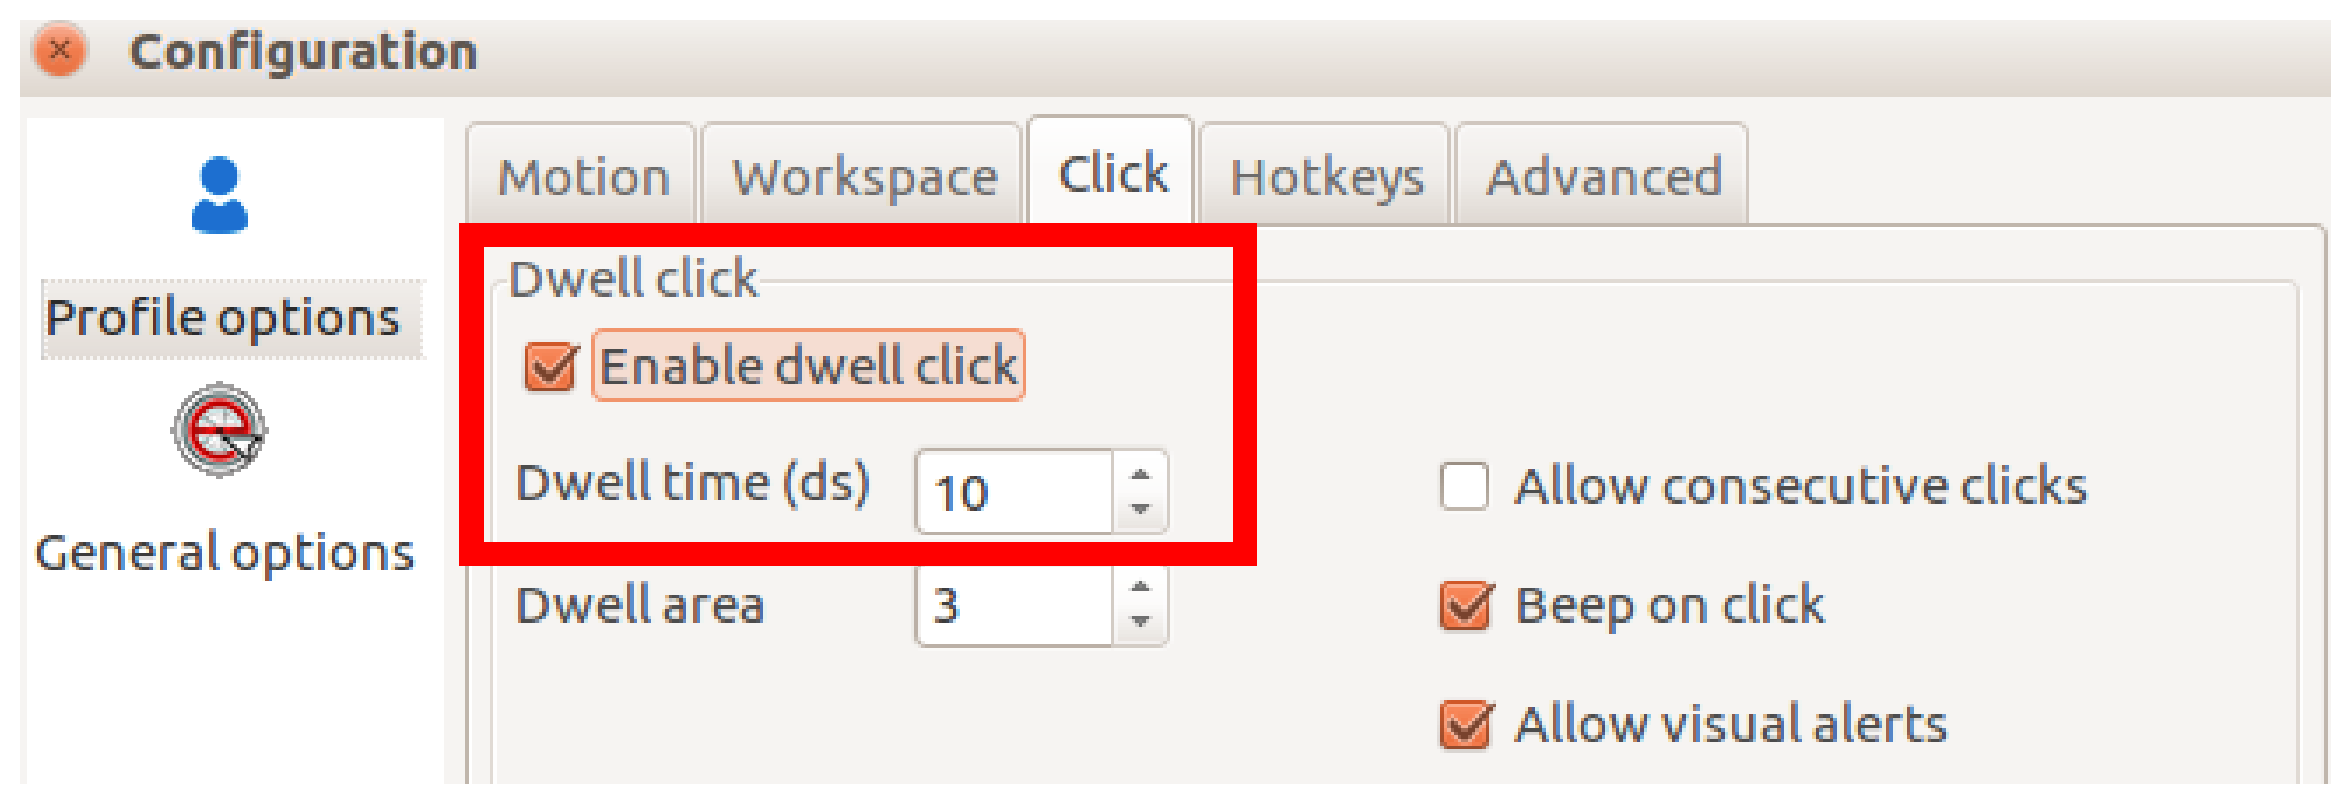
\includegraphics[width=0.7\linewidth]{fig/eviacamclick}
	\caption{Configuração do \textit{dwell time}.}
	\label{fig:click}
	\end{minipage}
\end{figure}
 
Há também a possibilidade de configurar a velocidade de movimentação do cursor
do \textit{mouse}. A Figura~\ref{fig:mouse} mostra, destacado em azul, a
configuração da velocidade do ponteiro nos eixos X e Y. O valor padrão é 10.

\begin{figure}[!h]
	\centering
	\begin{minipage}[c]{\textwidth}
	\centering
	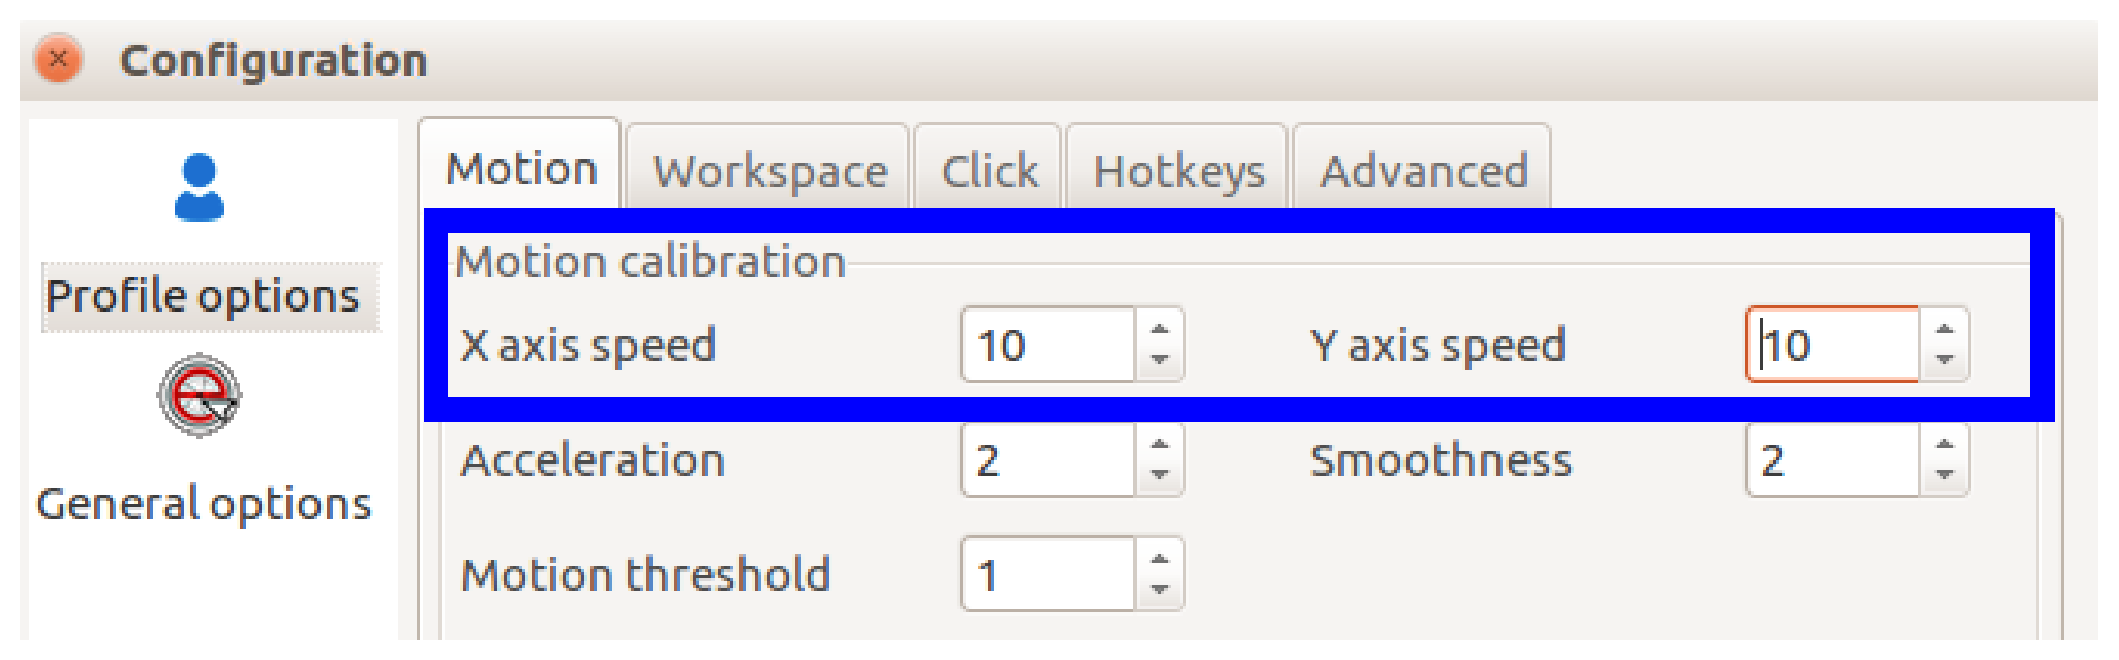
\includegraphics[width=0.7\linewidth]{fig/EviacamConfiguration}
	\caption{Configuração da velocidade de movimento do cursor do \textit{mouse}.}
	\label{fig:mouse}
	\end{minipage}
\end{figure}

\end{section}

\end{chapter}
